General equation of circle is 
\begin{align}
{\vec{x}^T\vec{x}} + 2\vec{u}^T\vec{x} + f = 0
\end{align}
 Taking equation of the first circle to be,
 \begin{align}
 \norm{\vec{x}}^2 + 2\vec{u}_1^T\vec{x} + f_1 = 0\label{eq:solutions/1/2.1.1}\\
 {\vec{x}^{T}\vec{x}}-4=0 \label{eq:solutions/1/2.1.2}\\
 \vec{u_1}=\myvec{0\\0}\\
 f_1=-4\\
\vec{O_1}=\myvec{0\\0}
 \end{align}
Taking equation of the second circle to be,
\begin{align}
  \norm{\vec{x}-\myvec{2\\0}}^2=2^2\\
  {\vec{x}^{T}\vec{x}+2\vec{u_2}^T\vec{x}}=0 \label{eq:solutions/1/2.2.2}\\
  \vec{u_2}=\myvec{-2\\0}\\
 f_2=0\\
 \vec{O_2}=\myvec{2\\0}
  \end{align}
 Now,Subtracting equation \eqref{eq:solutions/1/2.2.2} from \eqref{eq:solutions/1/2.1.2} We get,
 \begin{align}
 \vec{x}^T\vec{x}-2\vec{u_2}^T\vec{x}+f_1-\vec{x}^{T}\vec{x}=0\\
 2\vec{u}^{T}\vec{x}=-4\\
 \myvec{-4&0}\vec{x}=-4
 \end{align}
 Which can be written as:-
 \begin{align}
 \myvec{1&0}\vec{x}=1\\
 \vec{x}=\myvec{1 \\ 0} + \lambda \myvec{0\\1}\\
\vec{x}=\vec{q}+\lambda\vec{m}\label{eq:solutions/1/2.2.10}\\
\vec{q}=\myvec{1 \\ 0} \\
\vec{m}=\myvec{0\\1}
  \end{align}
 Substituting \eqref{eq:solutions/1/2.2.10} in \eqref{eq:solutions/1/2.1.1}
  \begin{align}
 \norm{\vec{x}}^2 + 2\vec{u}_1^T\vec{x} + f_1 = 0\\
 \norm{\vec{q}+\lambda\vec{m}}^2 + f_1 = 0\\
 (\vec{q}+\lambda \vec{m})^T(\vec{q}+\lambda \vec{m})+f_1=0\\
 \vec{q}^T(\vec{q}+\lambda \vec{m})+\lambda \vec{m}^T(\vec{q}+\lambda \vec{m})+f_1=0\\
 \norm{\vec{q}}^2+\lambda\vec{q}^T\vec{m}+\lambda\vec{m}^T\vec{q}+\lambda^2\norm{\vec{m}}^2+f_1=0\\
 \norm{\vec{q}}^2+2\lambda\vec{q}^T\vec{m}+\lambda^2\norm{\vec{m}}^2+f_1=0 \\
\lambda(\lambda\norm{\vec{m}}^2+2\vec{q}^T\vec{m})=-f_1-\norm{\vec{q}}^2\\
\lambda^2\norm{\vec{m}}^2=-f_1-\norm{\vec{q}}^2\\
\lambda^2=\frac{-f_1-\norm{\vec{q}}^2}{\norm{\vec{m}}^2}\\
\lambda^2=3\\
 \lambda=+\sqrt{3},-\sqrt{3}
 \end{align}
Substituting the value of $\lambda$ in\eqref{eq:solutions/1/2.2.10}
\begin{align}
\vec{x}=\vec{q}+\lambda\vec{m}\\
\vec{A}=\myvec{1\\\sqrt{3}}\\
\vec{B}=\myvec{1\\-\sqrt{3}}
 \end{align} 
 Now finding the direction vector $ \vec{m}_{O_1A}$,$\ \vec{m}_{O_1B}$,$ \vec{m}_{O_2A}$ and $\ \vec{m}_{O_2B}$.
\begin{align}
\vec{m}_{O_1A}=\myvec{0\\0}-\myvec{1\\\sqrt{3}}=\myvec{-1\\-\sqrt{3}}\\
\vec{m}_{O_1B}=\myvec{0\\0}-\myvec{1\\-\sqrt{3}}=\myvec{-1\\\sqrt{3}}\\
\vec{m}_{O_2A}=\myvec{2\\0}-\myvec{1\\\sqrt{3}}=\myvec{1\\-\sqrt{3}}\\
\vec{m}_{O_2B}=\myvec{2\\0}-\myvec{1\\-\sqrt{3}}=\myvec{1\\\sqrt{3}}
\end{align}
Now finding the angle $\angle{O_1AB}$.
\begin{align}
    \vec{m}_{O_1A}^T \vec{m}_{O_1B}=\norm{ \vec{m}_{O_1A}}\norm{\vec{m}_{O_1B}}\cos\theta_1\\
    \frac{\vec{m}_{O_1A}^T \vec{m}_{O_1B}}{\norm{ \vec{m}_{O_1A}}\norm{\vec{m}_{O_1B}}}
    =\cos\theta_1\\
     \frac{-2}{4}=\cos\theta_1\\
    \frac{-1}{2}=\cos\theta_1\\
    \theta_1=120^{\circ}
\end{align}
Now finding the angle $\angle{O_2AB}$.
\begin{align}
   \vec{m}_{O_2A}^T \vec{m}_{O_2B}=\norm{ \vec{m}_{O_2A}}\norm{\vec{m}_{O_2B}}\cos\theta_2\\
    \frac{\vec{m}_{O_2A}^T \vec{m}_{O_2B}}{\norm{ \vec{m}_{O_2A}}\norm{\vec{m}_{O_2B}}}
    =\cos\theta_2\\
     \frac{-2}{4}=\cos\theta_2\\
    \frac{-1}{2}=\cos\theta_2\\
    \theta_2=120^{\circ}
\end{align}
Finding area of $\bf{O_1AB}$ and $\bf{O_2AB}$.
 \begin{align}
A_{O_1AB}=\frac{\theta_1}{360}r^2-\frac{1}{2}2\sqrt{3}\\
=\frac{120}{360}4\pi-\frac{1}{2}2\sqrt{3}\\
A_{O_2AB}=\frac{\pi\theta_2}{360}r^2-\frac{1}{2}2\sqrt{3}\\
=\frac{120}{360}4\pi-\frac{1}{2}2\sqrt{3}
\end{align}
Area of  $\bf{O_1AO_2B}$
\begin{align}
A_{O_1AO_2B}=\frac{120}{360}4\pi-\frac{1}{2}2\sqrt{3}+\frac{120}{360}4\pi-\frac{1}{2}2\sqrt{3}\\
=\frac{8\pi}{3}-2\sqrt{3}
\end{align}
  \begin{figure}[h!]
	\centering
	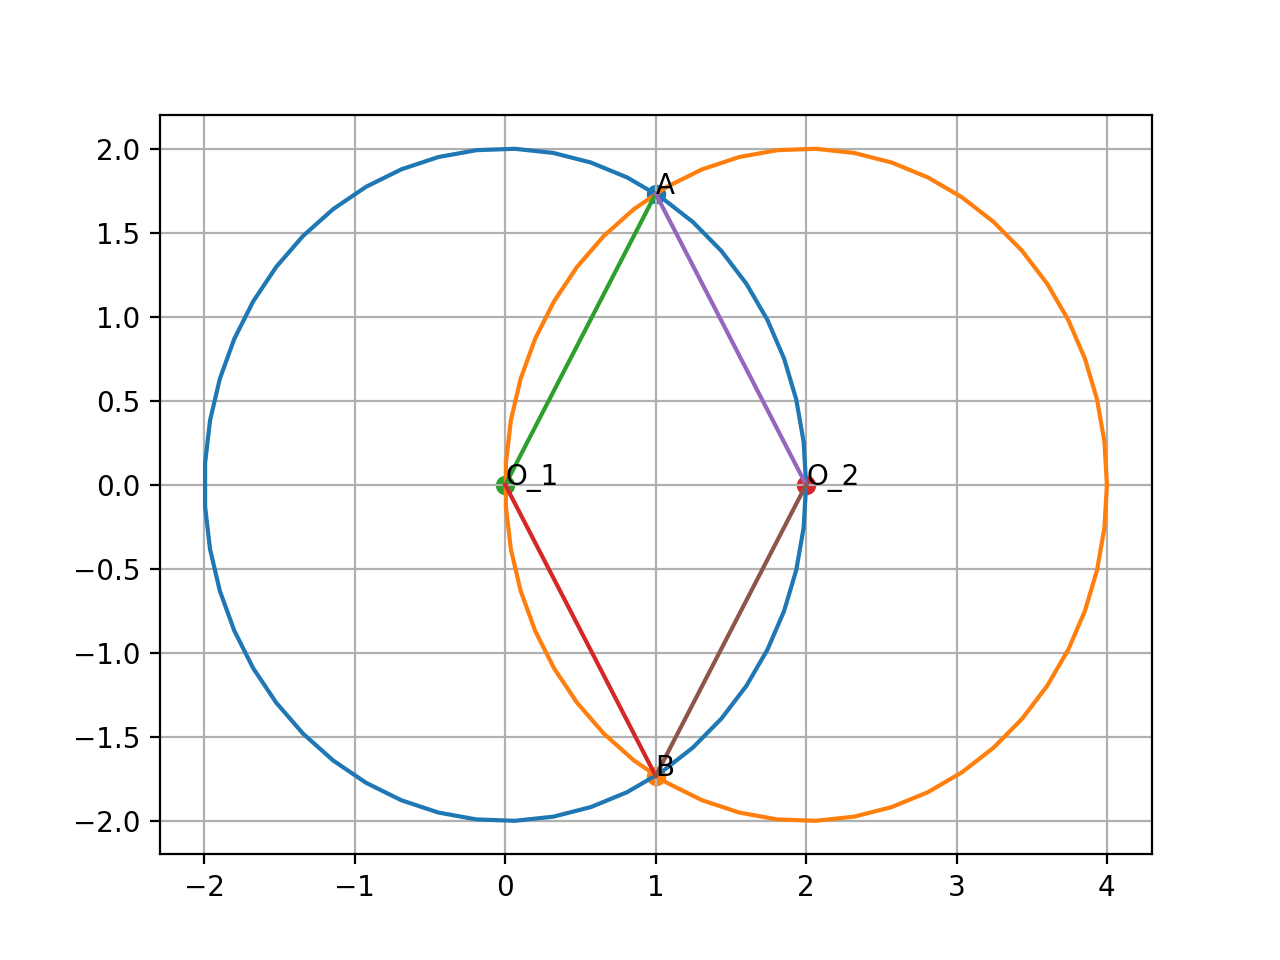
\includegraphics[width=\columnwidth]{./solutions/1/1/Assignment_5.png}
	\caption{Figure depicting intersection points of circle}
	\label{eq:solutions/1/myfig:solutions/1/}
\end{figure}
 
